\documentclass[12pt,letterpaper]{article}

\usepackage[spanish, es-nodecimaldot]{babel}
\usepackage[utf8]{inputenc}
\usepackage[T1]{fontenc}
\usepackage{lmodern}
\usepackage{amssymb, amsmath}
\usepackage{geometry}
\geometry{margin=1in}
\usepackage{setspace}
\onehalfspacing
\usepackage{float}
\setlength{\parskip}{0.25em}
\usepackage{graphicx}
\usepackage{xcolor}
\usepackage{tabularx}
\usepackage{booktabs}
\renewcommand{\arraystretch}{1.25}
\setlength{\tabcolsep}{8pt}
\newcolumntype{Y}{>{\raggedright\arraybackslash}X}
\usepackage{xurl}
\usepackage{hyperref}
\usepackage{enumitem}
\usepackage{titlesec}
\usepackage{verbatim}
\titleformat{\section}{\large\bfseries}{\thesection.}{0.5em}{}
\titleformat{\subsection}{\normalsize\bfseries}{\thesubsection}{0.5em}{}
\titleformat{\subsubsection}{\normalsize\itshape}{\thesubsubsection}{0.5em}{}
\usepackage{fancyhdr}
\pagestyle{fancy}
\fancyhf{}

\newcommand{\universidad}{Pontificia Universidad Javeriana}
\newcommand{\facultad}{Facultad de Ingeniería}
\newcommand{\carrera}{Ingeniería de Sistemas}
\newcommand{\curso}{Visualización de Datos}
\newcommand{\proyecto}{Análisis y visualización de delitos en Bogotá}
\newcommand{\subtitulo}{Entrega Final}
\newcommand{\profesor}{Laura Gomez}
\newcommand{\autores}{Luis Gutiérrez \\ Emilio Vargas \\ Santiago Suarez}
\newcommand{\fechaentrega}{Bogotá, Mayo de 2026}
\newcommand{\abreviaturaCurso}{Visualización de Datos}

\hypersetup{
  colorlinks=true,
  linkcolor=black,
  urlcolor=blue,
  citecolor=black,
  pdfauthor={\autores},
  pdftitle={\proyecto}
}

\fancyhead[L]{\small \abreviaturaCurso}
\fancyhead[R]{\small \universidad}
\fancyfoot[C]{\thepage}

\sloppy

\begin{document}

\begin{titlepage}
  \centering
  \vspace*{0.5cm}
  \includegraphics[width=5cm]{logo_javeriana.png}\par
  \vspace{0.5cm}
  {\Large \universidad \par}
  {\large \facultad \par}
  {\large \carrera \par}
  \vspace{2.0cm}
  {\Large \textbf{\proyecto}\par}
  \vspace{0.5cm}
  {\large \textbf{\subtitulo}\par}
  \vspace{0.8cm}
  {\large \textbf{Asignatura:} \curso\par}
  \vspace{0.8cm}
  {\large \textbf{Autores:}\par}
  {\large \autores\par}
  \vspace{0.8cm}
  {\large \textbf{Profesor:} \profesor\par}
  \vfill
  {\large \fechaentrega\par}
\end{titlepage}

\setcounter{page}{1}
\tableofcontents
\newpage

%==============================================================================
\section{Introducción}
%==============================================================================

La seguridad ciudadana es uno de los principales desafíos en ciudades como Bogotá, donde los delitos de alto impacto y los hurtos a personas afectan tanto la calidad de vida como la percepción de seguridad de la población. En este contexto, el análisis y la visualización de datos se convierten en herramientas clave para comprender el comportamiento de la criminalidad y apoyar la toma de decisiones estratégica. Por ello, el presente proyecto busca, integrando información proveniente de registros oficiales, llamadas a la línea 123 y datos geográficamente de las UPZ. A través de herramientas de análisis exploratorio y dashboards interactivos, se pretende identificar patrones temporales y especiales, zonas críticas y tendencias relevantes que faciliten la priorización de recursos y el fortalecimiento de las estrategias de seguridad ciudadana.

%==============================================================================
\section{Contexto}
%==============================================================================

\subsection{Sector de seguridad ciudadana}

El proyecto se desarrolla en el sector de seguridad ciudadana, enfocado en el análisis de delitos de alto impacto y hurto a personas en Bogotá. Este sector busca reducir la criminalidad y mejorar la calidad de vida mediante el uso de información y herramientas analíticas que permiten entender mejor el comportamiento del delito. Se trata de situaciones que impactan cómo las personas perciben la seguridad, y son situaciones que demandan acciones operativas permanentes tanto de monitoreo como de reacción. El propósito principal es identificar patrones en el espacio y el tiempo, comprender los aumentos repentinos y las variaciones en los tipos de delito, y convertir ese análisis en una asignación zonal prioritaria. Así, es posible tomar decisiones fundamentadas en información real sobre la manera en que se distribuyen los recursos y los programas gubernamentales orientados a garantizar la seguridad en Bogotá.

\subsection{Organización: OLSC-Bogotá}

Inicialmente se delimita el alcance del análisis en la visualización en las UPZ como unidad base. Los conjuntos de datos seleccionados permiten principalmente calcular tasas por cada 100 mil habitantes (cuando se dispone de población), densidad por kilómetro cuadrado, identificar tendencias, variaciones por día y hora, correlaciones entre los llamados de emergencia al 123 y los delitos, y comparar antes y después de intervenciones.

Con base en lo anterior, se define la organización en donde aplicar el proyecto: el Observatorio Local de Seguridad y Convivencia de Bogotá (OLSC-Bogotá), cuyo objetivo es ordenar, documentar y analizar fuentes de información ya existentes, articular sus clasificaciones y generar productos de inteligencia aplicada. Entre estos productos se incluyen informes ejecutivos mensuales, seguimiento a las modalidades delictivas en Bogotá, e identificación de señales de demanda ciudadana provenientes de la línea 123, con el fin de alimentar los comités locales de seguridad. La unidad de análisis prioritaria es la UPZ, lo cual se alinea con la estructura de planeación urbana del Distrito y los planes de acción zonales.

%==============================================================================
\section{Problema}
%==============================================================================

En la organización seleccionada, existe un flujo de trabajo compuesto de cuatro etapas:

\begin{enumerate}[label=\roman*.]
    \item Adición y estandarización de datos (incluyendo fechas, territorios, categorías y dominios)
    \item Modelado relacional y dimensional con adición de variables temporales y espaciales
    \item Análisis exploratorio para la evaluación de completitud, consistencia y patrones de los datos
    \item Difusión de resultados mediante paneles interactivos y boletines de alerta.
\end{enumerate}

Este proceso y los análisis que realizan tienen como usuarios destino a coordinadores y analistas de seguridad zonales, así como actores académicos o comunitarios que necesiten soluciones que sean medibles y comparables en el tiempo y en el espacio. Adicionalmente, la función que realiza el OLSC en colaboración con las entidades gubernamentales es la de recopilar sus datos y utilizarlos para liderar soluciones en la gestión de la seguridad y las emergencias.

Teniendo en cuenta todo lo mencionado, se detectan ciertas necesidades de la organización:

\begin{itemize}
    \item Integración de fuentes específicas y dispersas para relacionar los incidentes reportados y recopilados en bases de datos con lo que se registra como delito.
    \item Visualizaciones funcionales con múltiples filtros específicos tanto por UPZ, franjas horarias y mapas.
    \item Reportes formales para análisis por juntas de acción comunal y para el seguimiento de las intervenciones pertinentes.
\end{itemize}

\section{Objetivos del proyecto}

\subsection{Objetivo general}

Desarrollar un sistema de análisis y visualización de datos sobre hurtos a personas en Bogotá para apoyar la toma de decisiones estratégicas en el ámbito de seguridad en la ciudad.

\subsection{Objetivos específicos}

\begin{enumerate}
    \item Recopilar, limpiar y modelar conjuntos de datos provenientes de diversas fuentes (Datos Abiertos Bogotá, NUSE 123).
    \item Desarrollar indicadores clave para analizar patrones temporales, diferencias entre territorios y relaciones entre los delitos y las solicitudes de las personas.
    \item Crear dashboards interactivos que permitan visualizar la información con filtros ajustables y mapas a nivel de UPZ.
\end{enumerate}

\section{Objetivos de analítica y visualización}

\begin{enumerate}
    \item \textbf{Prioridad de zonas por UPZ:} Identificar la concentración de la demanda ciudadana ante emergencias por UPZ, y contrastarla con el comportamiento del hurto a nivel urbano para orientar la asignación de recursos.
    \item \textbf{Ritmos semanales y franjas horarias:} Analizar la distribución de incidentes atendidos por la línea de emergencias según día de la semana y franjas horarias, e identificar en el registro oficial de hurtos los momentos en que conviene reforzar vigilancia y patrullaje. 
    \item \textbf{Tendencia temporal:} Desarrollar series temporales de la incidencia del hurto y de la demanda ante la línea de emergencias para identificar evolución, estacionalidad y posibles puntos de cambio. 
    \item \textbf{Evaluación de intervenciones:} Comparar indicadores de incidencia y de demanda ciudadana en periodos de fechas antes y después a intervenciones de seguridad, reales o simuladas. 
    \item \textbf{Relación demanda ciudadana y registro oficial:} Explorar la relación entre la demanda ante la línea de emergencias y el comportamiento del hurto registrado, e identificar en qué zonas esa relación es más evidente.
\end{enumerate}

%==============================================================================
\section{Preguntas generadoras}
%==============================================================================

\begin{enumerate}
    \item ¿En qué UPZ se concentran los eventos de inseguridad de manera crítica, y cuáles deberían priorizarse para la asignación de recursos gubernamentales?
    \item ¿Cuáles son los días de la semana y las franjas horarias donde se concentran los diferentes tipos de delito, y en qué momentos críticos conviene reforzar los recursos de vigilancia y patrullaje?
    \item ¿Cómo ha evolucionado la incidencia de cada tipo de delito en Bogotá, y cuáles han sido los cambios de tendencia que permiten evaluar el impacto de intervenciones futuras?
    \item ¿Las intervenciones de seguridad implementadas (reales o simuladas) han generado una reducción significativa en los indicadores clave como densidad delictiva, tasa por 100 mil habitantes o índice de franjas horarias críticas?
    \item ¿En qué categorías de delito y en qué UPZ la demanda ciudadana registrada a través de la línea 123 anticipa el comportamiento de los delitos formalmente denunciados?
\end{enumerate}

%==============================================================================
\section{Conjuntos de datos y proceso de preparación}
%==============================================================================

\subsection{Descripción de las fuentes}

El primer dataset utilizado corresponde a los registros de hurtos en Bogotá durante el año 2025. Este conjunto de datos contiene información detallada sobre los eventos de hurto, incluyendo variables como la fecha del hecho, el género de la víctima, el grupo etario, el tipo de arma o medio utilizado, el departamento, el municipio, el código DANE y la cantidad de casos reportados. Este dataset es fundamental para el proyecto, ya que permite analizar la dinámica de la criminalidad en la ciudad, identificar patrones temporales y segmentar los incidentes según características demográficas y contextuales.

Los conjuntos de datos utilizados están disponibles en las siguientes fuentes:
\begin{itemize}[noitemsep, topsep=0pt]
    \item Estadística delictiva (Policía Nacional de Colombia): \url{https://www.policia.gov.co/estadistica-delictiva}
    \item Delito de Alto Impacto (Datos Abiertos Bogotá): \url{https://datosabiertos.bogota.gov.co/dataset/delito-de-alto-impacto-bogota-d-c}
    \item Incidentes tramitados en el C4 -- NUSE (Datos Abiertos Bogotá): \url{https://datosabiertos.bogota.gov.co/dataset/incidentes/resource/30d65a8b-d0ed-4e95-977e-0d7cc2ea89ef}
\end{itemize}

El segundo dataset corresponde a las llamadas realizadas a la línea de emergencias 123 (C4). Este conjunto de datos incluye información sobre los incidentes reportados por la ciudadanía, tales como el tipo de evento, la fecha y hora de la llamada, la ubicación y en algunos casos una descripción del suceso. Este dataset aporta una perspectiva complementaria al análisis, ya que permite estudiar la percepción ciudadana de seguridad y contrastar con los registros oficiales de hurtos, facilitando la identificación de posibles diferencias entre los eventos reportados y los registrados.

El tercer dataset corresponde a la División Administrativa de Bogotá a nivel de Unidades de Planeamiento Zonal (UPZ). Contiene la delimitación espacial de cada UPZ, identificadores de zona y variables de apoyo para tasas y densidad. Su principal utilidad es georreferenciar la demanda ante la línea de emergencias y construir mapas por UPZ; el registro de hurtos de la Policía, en la versión utilizada, se analiza a nivel urbano y no se cruza territorialmente con esta capa.

\subsection{Preparación y limpieza de datos}

El proceso de preparación se ejecutó con \textbf{Python} (\texttt{pandas}, \texttt{geopandas}) mediante el script \texttt{DATASETS/scripts/clean\_datasets.py}, que automatiza la depuración de las fuentes principales. Los archivos resultantes se organizaron en dos carpetas: \texttt{DATASETS/data/}, con las tablas de hechos y la capa geográfica, y \texttt{DATASETS/nuevas-tablas/}, con las tablas de dimensión para el modelo en Power~BI. Todos los archivos tabulares comparten separador de campo punto y coma (\texttt{;}) y codificación UTF-8.

\subsubsection{Hurtos a personas (\texttt{hurtos\_bogota\_2025.csv})}

La fuente original correspondía a un archivo CSV de la Policía Nacional con codificación \texttt{latin-1}, fechas en formato \texttt{d/m/aaaa} y separador \texttt{;}. Durante la revisión se identificó que el código DANE es único para todo el archivo (\texttt{11001000}, municipio de Bogotá), por lo que la geografía del hurto queda a \textbf{nivel urbano} y no por UPZ.

Las transformaciones aplicadas fueron:
\begin{itemize}[noitemsep, topsep=0pt]
    \item Conversión a UTF-8 y normalización de nombres de columnas.
    \item Parseo de \texttt{fecha\_hecho} a formato ISO (\texttt{YYYY-MM-DD}) y creación de variables temporales (\texttt{anio}, \texttt{mes}, \texttt{dia\_semana}, \texttt{nombre\_dia}).
    \item Limpieza de categorías (\texttt{genero}, \texttt{agrupa\_edad}, \texttt{armas\_medios}): recorte de espacios y reemplazo de vacíos por \texttt{SIN\_DATO}.
    \item Campo \texttt{nivel\_geografico} = \texttt{municipio}.
    \item Agregación de registros repetidos por combinación de fecha, perfil de víctima y arma o medio, sumando el campo \texttt{cantidad}, con el fin de conservar el total de casos y reducir redundancia para el dashboard.
\end{itemize}

\textbf{Resultado:} de 100\,017 filas en origen a 3\,982 filas limpias; la suma de \texttt{cantidad} se mantiene en 100\,017. No se descartaron fechas inválidas.

\subsubsection{Incidentes línea 123 / C4 (\texttt{Llamadas123C4.csv})}

El recurso de Datos Abiertos Bogotá se entregó en JSON (estructura \texttt{fields} + \texttt{records}). Se transformó a CSV para su importación en Power~BI. Entre los hallazgos de calidad destacan: coordenadas con coma decimal, códigos sentinela de localización (\texttt{UPZ999}, \texttt{UPZ99x}), registros con latitud/longitud en cero y duplicados por \texttt{id\_incidente}.

Las transformaciones aplicadas fueron:
\begin{itemize}[noitemsep, topsep=0pt]
    \item Aplanado del JSON a tabla y estandarización de nombres de columnas.
    \item Fecha en ISO; coordenadas numéricas con punto decimal.
    \item Normalización de \texttt{cod\_upz} (mayúsculas) y de textos (\texttt{nombre\_dia}, \texttt{localidad}).
    \item Variables de control: \texttt{sin\_localizacion}, \texttt{coord\_valida} y \texttt{upz\_valida} (validación contra el catálogo de UPZ y un bounding box aproximado de Bogotá).
    \item Eliminación de duplicados por \texttt{id\_incidente}, conservando el registro con mejor georreferenciación.
    \item Supresión del archivo JSON original tras generar el CSV depurado.
\end{itemize}

\textbf{Resultado:} de 33\,298 filas en origen a 30\,431 filas (2\,867 duplicados eliminados). Aproximadamente el 10,7\,\% de los registros quedó marcado como \texttt{sin\_localizacion}; 27\,181 cuentan con coordenadas válidas y 27\,182 con UPZ válida frente al catálogo espacial. El periodo cubre los años 2020 a 2025.

\subsubsection{División UPZ (\texttt{DAIUPZ.geojson})}

El archivo administrativo se recibió en formato TopoJSON, poco compatible con visualizaciones estándar en Power~BI. Se convirtió a \textbf{GeoJSON} en referencia \texttt{EPSG:4326}, conservando únicamente atributos analíticos: \texttt{objectid}, \texttt{cod\_upz}, \texttt{nombre\_upz}, \texttt{poblacion\_proxy} (derivado de \texttt{CMHPTOTAL}) y \texttt{area\_km2} (cálculo en \texttt{EPSG:9377}). Se exportaron 116 polígonos; el archivo TopoJSON original se eliminó tras la conversión.

\subsubsection{Tablas de dimensión (\texttt{nuevas-tablas/})}

Para soportar un esquema tipo estrella en Power~BI, se generaron catálogos independientes, alineados con el modelo de referencia del curso:
\begin{itemize}[noitemsep, topsep=0pt]
    \item \texttt{Calendar.csv}: calendario continuo del 1 de enero de 2020 al 31 de diciembre de 2025 (2\,192 días, hora \texttt{00:00:00}).
    \item \texttt{Localidad.csv}: códigos y nombres de localidad de Bogotá (incluye categorías especiales como \texttt{SIN LOCALIZACION}).
    \item \texttt{Genero.csv} y \texttt{ArmaMedio.csv}: dominios de género y arma o medio para relacionar con hurtos.
    \item \texttt{FranjaHoraria.csv}: ocho franjas horarias y su periodo del día (\texttt{MAÑANA}, \texttt{TARDE}, \texttt{NOCHE}, \texttt{MADRUGADA}).
\end{itemize}

\subsubsection{Control de calidad y limitaciones}

\begin{table}[H]
  \centering
  \caption{Resumen de control de calidad tras la limpieza.}
  \label{tab:qc-datasets}
  \small
  \begin{tabularx}{\linewidth}{lXX}
    \toprule
    \textbf{Conjunto} & \textbf{Registros finales} & \textbf{Observación principal} \\
    \midrule
    Hurtos 2025 & 3\,982 (100\,017 casos) & Solo nivel municipio; sin franja horaria \\
    Llamadas 123 & 30\,431 & Georreferenciación por UPZ; muestra homogénea en tipo de incidente \\
    UPZ (GeoJSON) & 116 polígonos & Población proxy, no censo oficial 2025 \\
    Calendario & 2\,192 fechas & Cobertura 2020--2025 \\
    \bottomrule
  \end{tabularx}
\end{table}

Entre las \textbf{limitaciones} que condicionan el análisis y deben declararse en las visualizaciones se incluyen: (i)~el hurto no se desagrega por UPZ con la fuente de Policía utilizada; (ii)~la línea de emergencias, en la muestra trabajada, corresponde predominantemente a un mismo tipo de incidente, por lo que no representa todo el espectro de la demanda ciudadana; (iii)~\texttt{poblacion\_proxy} sirve para tasas relativas entre UPZ, pero no equivale a proyección oficial de habitantes; (iv)~indicadores de intervención requieren fechas definidas externamente al conjunto de datos. Las tasas por 100\,000 habitantes y la densidad se calcularán en Power~BI mediante medidas DAX, apoyadas en \texttt{poblacion\_proxy} y \texttt{area\_km2}.

\subsection{Integración de los conjuntos de datos}

La integración se plantea como un \textbf{modelo estrella} para Power~BI. Las tablas de hechos son \texttt{hurtos\_bogota\_2025} (registro oficial agregado) y \texttt{Llamadas123C4} (demanda ciudadana georreferenciada). La dimensión espacial principal es \texttt{DAIUPZ.geojson}, relacionada con las llamadas mediante \texttt{cod\_upz}. Las dimensiones \texttt{Calendar}, \texttt{Localidad}, \texttt{FranjaHoraria}, \texttt{Genero} y \texttt{ArmaMedio} unifican dominios temporales, territoriales y categóricos.

Las relaciones activas son:
\begin{itemize}[noitemsep, topsep=0pt]
    \item \texttt{Calendar[Date]} con \texttt{fecha\_hecho} y con \texttt{fecha} (llamadas).
    \item \texttt{Genero} y \texttt{ArmaMedio} con la tabla de hurtos.
    \item \texttt{Localidad} y \texttt{DAIUPZ} con la tabla de llamadas (\texttt{cod\_localidad}, \texttt{cod\_upz}).
    \item \texttt{FranjaHoraria} con \texttt{rango\_hora} en llamadas.
\end{itemize}

La tabla de hurtos \textbf{no} se relaciona con UPZ ni localidad en esta versión del modelo, dado el código DANE municipal único. El cruce entre demanda ciudadana y hurto se realiza principalmente por la dimensión temporal (y, en exploración, por comparación de patrones territoriales de llamadas frente a indicadores de hurto a nivel ciudad). Este diseño responde a las preguntas generadoras reformuladas del proyecto, manteniendo trazabilidad entre lo que permiten los datos y lo que se muestra en cada página del dashboard.

%==============================================================================
\section{Modelo lógico de datos final}
%==============================================================================

\subsection{Cambios respecto a la primera entrega}

\textit{[Pendiente: describir ajustes al modelo (nuevas entidades, atributos, relaciones o correcciones) derivados del trabajo de integración y limpieza.]}

\subsection{Descripción del modelo}

El modelo lógico de datos propuesto tiene como objetivo integrar información proveniente de diferentes fuentes para permitir el análisis del fenómeno de seguridad en Bogotá desde una perspectiva temporal, demográfica y geográfica. Para ello, se definieron cuatro entidades principales: \textbf{HECHOS-HURTO, LLAMADAS-123, UBICACION y UPZ,} las cuales se relacionan entre sí para estructurar la información de manera coherente y facilitar su análisis.

La entidad \textbf{HECHOS-HURTO} representa los registros oficiales de hurtos y constituye una de las tablas principales del modelo. En esta se almacenan variables clave como la fecha del hecho, el género de la víctima, el grupo etario, el tipo de arma utilizada y la cantidad de casos. Además, incluye el campo \textbf{codigo-dane}, que permite relacionar cada registro con su respectiva ubicación geográfica.

Por su parte, la entidad \textbf{LLAMADAS-123} contiene la información correspondiente a los reportes ciudadanos realizados a la línea de emergencias. Esta tabla incluye datos como la fecha del incidente, el tipo de evento reportado y su ubicación, también referenciada mediante el codigo-dane. Esta entidad complementa el análisis al aportar una visión desde la percepción ciudadana, permitiendo contrastar los datos oficiales con los reportes realizados por la comunidad.

La entidad \textbf{UBICACION} actúa como una tabla intermedia que centraliza la información geográfica, incluyendo el municipio, el departamento y la referencia a la UPZ correspondiente. Esta entidad es clave dentro del modelo, ya que permite unificar la información espacial de los distintos datasets y establecer relaciones entre ellos a través del codigo-dane.

Como último se usa la entidad \textbf{UPZ} que contiene la información geográfica detallada de las Unidades de Planeamiento Zonal, incluyendo su identificador, nombre y geometría. Esta tabla permite realizar análisis espaciales más específicos y facilita la construcción de visualizaciones geográficas, como mapas de calor o distribuciones por zonas.

En cuanto a las relaciones, tanto la entidad \textbf{HECHOS-HURTO} como \textbf{LLAMADAS-123} se conectan con \textbf{UBICACION} mediante una relación de muchos a uno, ya que múltiples registros pueden pertenecer a una misma ubicación. A la vez, \textbf{UBICACION} se relaciona con \textbf{UPZ} también en una relación de muchos a uno, permitiendo agrupar diferentes ubicaciones dentro de una misma zona geográfica.

\begin{figure}[H]
  \centering
  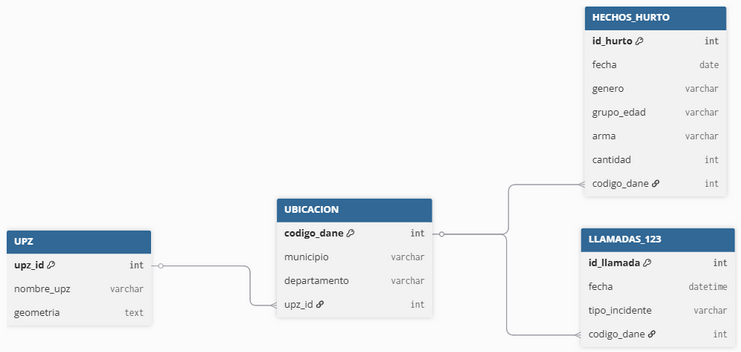
\includegraphics[width=16cm]{modelo-datos.png}
  \caption{Modelo lógico de datos del proyecto.}
  \label{fig:modelo-datos}
\end{figure}

%==============================================================================
\section{Registro de la visualización análoga en vivo}
%==============================================================================

\subsection{Diseño de la actividad}

\textit{[Pendiente: qué se observó o recolectó, dónde, cuándo y con qué protocolo.]}

\subsection{Evidencias}

\textit{[Pendiente: insertar fotografías, notas de campo y registros de la actividad.]}

\subsection{Resultados}

\textit{[Pendiente: hallazgos cuantitativos y cualitativos de la recolección en vivo.]}

\subsection{Reflexión metodológica}

\textit{[Pendiente: utilidad de la técnica, limitaciones (sesgo, muestra, horario, cobertura) y comparación con datos oficiales o del 123.]}

\subsection{Integración al análisis del proyecto}

\textit{[Pendiente: cómo los resultados de la visualización análoga alimentan preguntas generadoras u objetivos de analítica.]}

%==============================================================================
\section{Reporte Ejecutivo}
%==============================================================================

\textit{[Pendiente: herramienta utilizada, enlace de acceso y descripción general del tablero.]}

\subsection{Pantallas por objetivo de analítica}

\textit{[Pendiente: mínimo una pantalla por cada objetivo de analítica. Incluir capturas y breve interpretación.]}
\begin{itemize}
    \item \textbf{Objetivo 1 -- Prioridad de zonas por UPZ:} [nombre de pantalla / captura].
    \item \textbf{Objetivo 2 -- Ritmos semanales y franjas horarias:} [nombre de pantalla / captura].
    \item \textbf{Objetivo 3 -- Tendencia temporal por tipo de delito:} [nombre de pantalla / captura].
    \item \textbf{Objetivo 4 -- Evaluación de intervenciones:} [nombre de pantalla / captura].
    \item \textbf{Objetivo 5 -- Línea 123 como alerta temprana:} [nombre de pantalla / captura].
\end{itemize}

\subsection{Filtros dinámicos}

\textit{[Pendiente: documentar al menos cuatro filtros por categorías, por ejemplo UPZ, tipo de delito, periodo y franja horaria.]}

%==============================================================================
\section{Conclusiones y recomendaciones}
%==============================================================================

\subsection{Conclusiones}

\textit{[Pendiente: conclusiones vinculadas a preguntas generadoras y objetivos de analítica.]}

\subsection{Recomendaciones}

\textit{[Pendiente: recomendaciones operativas para el OLSC-Bogotá y actores de seguridad local.]}

%==============================================================================
\section{Lecciones aprendidas}
%==============================================================================

\textit{[Pendiente: reflexión sobre el proceso técnico, el trabajo en equipo, limitaciones del estudio y trabajo futuro.]}

%==============================================================================
\section{Anexos}
%==============================================================================

\textit{[Pendiente: listar y entregar los archivos adjuntos requeridos por el enunciado.]}
\begin{itemize}
    \item Datasets procesados: carpeta \texttt{DATASETS/data/} (hechos y UPZ) y \texttt{DATASETS/nuevas-tablas/} (dimensiones); script \texttt{DATASETS/scripts/clean\_datasets.py}.
    \item Modelo de datos: \texttt{[diagrama, DDL o archivo del modelo]}.
    \item Dashboard / visualizador: \texttt{[archivo .pbix, .twbx, URL, etc.]}.
    \item Reporte ejecutivo en PDF: \texttt{[nombre del archivo]}.
    \item Evidencias de visualización análoga: \texttt{[carpeta o archivos]}.
\end{itemize}

\addcontentsline{toc}{section}{Referencias}
\begin{thebibliography}{99}
\raggedright

\bibitem{cisc2025} 
Cisc. (2025). \textit{Estadística delictiva / Policía Nacional de Colombia}. Policía Nacional De Colombia. \url{https://www.policia.gov.co/estadistica-delictiva}

\bibitem{datosbog_altoimpacto}
\textit{Delito de Alto Impacto. Bogotá D.C. - Datos Abiertos Bogotá}. (s.f.). \url{https://datosabiertos.bogota.gov.co/dataset/delito-de-alto-impacto-bogota-d-c}

\bibitem{datosbog_nuse}
\textit{Incidentes Tramitados en el C4 - Numero Único de Seguridad y Emergencia. NUSE. Bogotá D.C. - Datos Abiertos Bogotá}. (s.f.). \url{https://datosabiertos.bogota.gov.co/dataset/incidentes/resource/30d65a8b-d0ed-4e95-977e-0d7cc2ea89ef}

\bibitem{alcaldia2024}
Alcaldía de Bogotá. (2024). \textit{En Bogotá, mi Ciudad, mi Casa contamos con el C4 para la seguridad y emergencias}. Bogota.gov.co. \url{https://bogota.gov.co/mi-ciudad/seguridad/en-bogota-mi-ciudad-mi-casa-contamos-con-el-c4-para-la-seguridad}

\bibitem{minjusticia}
Ministerio de Justicia y del Derecho. (s.f.). \url{https://www.minjusticia.gov.co/programas-co/politica-criminal/Paginas/SIPC-Tasa-de-Homicidios-Basada-en-reporte-de-homicidios-de-la-Policia-Nacional.aspx}

\end{thebibliography}

\end{document}